\documentclass{article}

\usepackage{amsfonts, amsmath,amssymb,amsthm}   % Paquetes de simbología matemática básica
\usepackage{lmodern,microtype,bm}     % Fuente y espaciado entre letras; lo deja bonito
\usepackage{dsfont, graphicx}
\usepackage{mathrsfs, halloweenmath,xcolor}
\usepackage{MnSymbol}
\usepackage{mathtools}
\usepackage{multicol,titlesec}
\usepackage[shortlabels]{enumitem}    % Continuar listas en mini-páginas distintas
\usepackage{physics}
\usepackage[english,spanish]{babel}   % Cambia los comandos de texto predeterminados (capítulos, 			                                        secciones, bibliografía, etc.) a español
\decimalpoint
\usepackage[style=mexican]{csquotes}  % Comillas y otros elementos de citación
\textwidth 16cm                       % Ancho
\oddsidemargin -0.0cm                 % Espacio de margen (como es formato de libro, los margenes se 		                                        declaran para páginas pares e impares
\usepackage[spanish]{todonotes}
\usepackage{xfrac}
\usepackage[unicode=true]{hyperref}

\newtheoremstyle{definicion}% name
{3pt}% Space above
{3pt}% Space below
{}% Body font
{}% Indent amount
{\color{blue}\bfseries}% Theorem head font
{.}% Punctuation after theorem head
{.5em}% Space after theorem head
{}%
\theoremstyle{definicion}
\newtheorem{definicion}{Def.}

\theoremstyle{definition}             % Con el paquete amsmath se pueden personalizar los estilos de
\newtheorem*{inst}{Instrucciones}

\theoremstyle{definition}             % Con el paquete amsmath se pueden personalizar los estilos de
\newtheorem{sol}{Solución}

\theoremstyle{definition}
\newtheorem{record}{Recordatorio}

\theoremstyle{definition}
\newtheorem{properties}{Propiedades}

\newtheoremstyle{observacion}% name
{3pt}% Space above
{3pt}% Space below
{}% Body font
{}% Indent amount
{\color{red}\bfseries}% Theorem head font
{.}% Punctuation after theorem head
{.5em}% Space after theorem head
{}%
\theoremstyle{observacion}
\newtheorem{obs}{Obs.}

\theoremstyle{definition}
\newtheorem{prop}{Proposición}

\theoremstyle{plain}
\newtheorem{lemma}{Lema}
\newtheorem{theorem}{Teorema}

\theoremstyle{definition}
\newtheorem{exe}{Ejemplo}

\newtheoremstyle{afirmacion}% name
{3pt}% Space above
{3pt}% Space below
{}% Body font
{}% Indent amount
{\color{green!40!black}\bfseries}% Theorem head font
{.}% Punctuation after theorem head
{.5em}% Space after theorem head
{}%
\theoremstyle{afirmacion}
\newtheorem{corollary}{Corolario}

\newtheoremstyle{notation}% name
{3pt}% Space above
{3pt}% Space below
{}% Body font
{}% Indent amount
{\color{magenta}\bfseries}% Theorem head font
{.}% Punctuation after theorem head
{.5em}% Space after theorem head
{}%
\theoremstyle{notation}
\newtheorem{notation}{Notación}

\theoremstyle{definition}
\newtheorem{eje}{Ejercicio}

\setlength{\parindent}{2em}           % Sangría
\setlength{\parskip}{0.5em}           % Espacio entre párrafos

\graphicspath{{./img}}

\title{\Huge{El plano euclidio}}
\author{Geometría Analítica I}
\date{\today}

\begin{document}
    \maketitle

    \section{El espacio vectorial \texorpdfstring{\(\mathbb{R}^{2}\)}{ℝ²}}

    En esta sección se introduce la herramienta algebraica básica para hacer geometría con parejas, ternas o \(n\)-adas de números.

    \begin{definicion}
        Dados dos vectores \(\vb*{u} = (x, y)\) y \(\vb{v} = (x^{\prime}, y^{\prime})\) en \(\mathbb{R}^{2}\), definimos su \textcolor{blue}{suma vectorial}, o simplemente suma, como el vector \(\vb*{u} + \vb*{v}\) que resulta de sumar componente a componente:

        \begin{equation*}
            \vb*{u} + \vb*{v} \coloneq (x + x^{\prime}, y + y^{\prime}).
        \end{equation*}

        Nótese que en cada coordenada, la suma que se usa es la suma usual de números reales.
    \end{definicion}

    La suma vectorial corresponde geométricamente a la regla del paralelogramo usada para encontrar la resultante de dos vectores. Esto es, se consideran los vectores como segmentos dirigidos que salen del origen y generan entonces un paralelogramo, y el vector que va del origen a la otra esquina es la suma.
    
    \begin{figure}[htb]
        \centering
        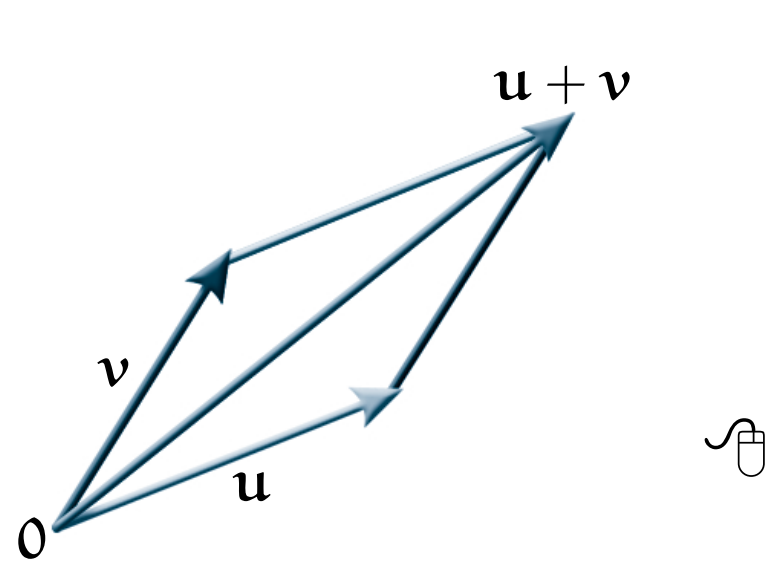
\includegraphics[scale=0.2]{1}
        \caption{Método del paralelogramos}
        \label{fig:paralelogramo}
    \end{figure}

    \begin{definicion}
        Dados un vector \(\vb*{u} = (x, y) \in \mathbb{R}^{2}\) y un número \(t \in \mathbb{R}\) se define la \textcolor{blue}{multiplicación escalar} \(t \vb*{u}\) como el vector que resulta de multiplicar cada componente del vector por el número:

        \begin{equation*}
            t \vb*{u} \coloneq (t x, t y).
        \end{equation*}

        Nótese que en cada coordenada la multiplicación que se usa es de los números reales.
    \end{definicion}

    \begin{obs}
        Notemos que \(t \vb*{u}\) para \(t > 1\) es, estrictamente hablando, una \textcolor{blue}{dilatación} de \(\vb*{u}\), y para \(0 < t < 1\), una \textcolor{blue}{contracción} del mismo. Además, para \(t < 0\), \(t \vb*{u}\) apunta en la dirección contraria, ya que, en particular, \((-1) \vb*{u} \eqqcolon - \vb*{u}\) es el vector que, como segmento dirigido, va del punto \(\vb*{u}\) al \(\vb*{0}\) y el resto se obtiene como dilataciones o contracciones de \(- \vb*{u}\).
    \end{obs}

    Las propiedades básicas de la suma vectorial y la multiplicación escalar se reúnen en el siguiente teorema, donde el vector \(\vb*{0} = (0, \dots, 0)\) es el llamado \textcolor{blue}{vector cero} que corresponde al origen, y, para cada \(x \in \mathbb{R}^{n}\), el vector \(-x \coloneq (-1)x\) se llama \textcolor{blue}{inverso aditivo} de \(x\).

    \begin{theorem}
        Para todos los vectores \(x,\ y,\ z \in \mathbb{R}^{n}\) y para todos los números \(s,\ t \in \mathbb{R}\) se cumple que:

        \begin{enumerate}[label = \textnormal{\Roman*)}]
            \item \((x + y) + z = x + (y + z)\)
            \item \(x + y = y + z\)
            \item \(x + \vb*{0} = x\)
            \item \(x + (-x) = \vb*{0}\)
            \item \(s(tx) = (st)x\)
            \item \(1x = x\)
            \item \(t(x + y) = tx + ty\)
            \item \((s + t)x = sx + tx\)
        \end{enumerate}
    \end{theorem}

    \begin{lemma}
        Si \(x \in \mathbb{R}^{2}\) y \(t \in \mathbb{R}\) son tales que \(tx = \vb*{0}\) entonces \(t = 0\) 0 \(x = \vb*{0}\).
    \end{lemma}

    \section{Líneas}

    Se nos pide describir el conjunto \(\mathcal{L}_{\vb*{v}} \coloneq \left\lbrace t\vb*{v} \in \mathbb{R}^{2} \mid t \in \mathbb{R}\right\rbrace\) donde \(\vb*{v} \in \mathbb{R}^{2}\). Es claro que que si \(\vb*{v} \neq \vb*{0}\), entonces \(\mathcal{L}_{\vb*{v}}\), al constar de todos los múltiplos escalares del vector \(\vb*{v}\), se dibuja como una recta que pasa por el origen (pues \(\vb*{0} = 0\vb*{0}\)) con la dirección de \(\vb*{v}\).

    \begin{definicion}
            Dados un punto \(\vb*{p}\) y un vector \(\vb*{v} \neq \vb*{0}\), la \textcolor{blue}{recta que pasa por} \(\vb*{p}\) \textcolor{blue}{con dirección} \(\vb*{v}\) es el conjunto

            \begin{equation*}
                \ell \coloneq \left\lbrace \vb*{p} + t\vb*{v} \mid t \in \mathbb{R}\right\rbrace.
            \end{equation*}

            Una \textcolor{blue}{recta} o \textcolor{blue}{línea} en \(\mathbb{R}^{2}\) es un subconjunto que tiene, para algún \(\vb*{p}\) y \(\vb*{v} \neq \vb*{0}\), la descripción anterior.
            A esta forma de definir una recta se le conoce como \textcolor{blue}{representación (o expresión) paramétrica}.
    \end{definicion}

    \begin{lemma}
        Dados dos puntos \(\vb*{p}\) y \(\vb*{q}\) en \(\mathbb{R}^{2}\), existe una recta que pasa por ellos.
    \end{lemma}
    \begin{proof}
        Si tuviéramos que \(\vb*{p} = \vb*{q}\), como  hay muchas rectas que pasan por \(\vb*{p}\), ya acabamos. Supongamos entonces que \(\vb*{p} \neq \vb*{q}\). Si tomamos a \(\vb*{p}\) como punto base para la recta que buscamos, bastará con encontrar un vector que nos lleve de \(\vb*{p}\) a \(\vb*{q}\), para tomarlo como dirección. Este es la diferencia \(\vb*{q} - \vb*{p}\), pues claramente

        \begin{equation*}
            \vb*{p} + (\vb*{q} - \vb*{p}) = \vb*{q},
        \end{equation*}

        de tal manera que si definimos \(\vb*{d} \coloneq \vb*{q} - \vb*{p}\), como dirección, la recta

        \begin{equation*}
            \ell \coloneq \left\lbrace \vb*{p} + t\vb*{d} \mid t \in \mathbb{R}\right\rbrace
        \end{equation*}

        (que sí es una recta pues \(\vb*{d} = \vb*{q} - \vb*{p} \neq \vb*{0}\)), es la que funciona. Con \(t = 0\) obtenemos que \(\vb*{p} \in \ell\), y con \(t = 1\) que \(\vb*{q} \in \ell\).
    \end{proof}

    \begin{obs}
        Obsérvese que cuando \(t\) toma valores entre \(0\) y \(1\), se obtienen puntos entre \(\vb*{p}\) y \(\vb*{q}\), así que al \textcolor{blue}{segmento} de \(\vb*{p}\) a \(\vb*{q}\), que denotaremos con \(\overline{\vb*{p}\vb*{q}}\), se debe definir como

        \begin{equation*}
            \overline{\vb*{p}\vb*{q}} \coloneq \left\lbrace \vb*{p} + t(\vb*{p} - \vb*{q}) \mid 0 \leq t \leq 1\right\rbrace.
        \end{equation*}

        Y la recta \(\ell\) que pasa por \(\vb*{p}\) y \(\vb*{q}\) se extiende ``indefinidamente'' a ambos lados del segmento \(\overline{\vb*{p}\vb*{q}}\), para \(t > 1\) del lado de \(\vb*{q}\) y para \(t < 0\) del lado de \(\vb*{p}\).
    \end{obs}

    \subsection{Coordenadas baricéntricas}

    Supongamos que \(\vb*{p}\) y \(\vb*{q}\) son puntos distintos del plano. Para cualquier \(t \in \mathbb{R}\) , se tiene que

    \begin{equation*}
        \vb*{p} + t(\vb*{q} - \vb*{p}) = \vb*{p} + t\vb*{q} - t\vb*{p} = (1 - t)\vb*{p} + t\vb{q}
    \end{equation*}

    al reagrupar los términos. Y esta última expresión, a su vez, se puede reescribir como 

    \begin{equation*}
        s\vb*{p} + t\vb*{q}\quad \text{con} \quad s + t = 1,
    \end{equation*}

    donde hemos introducido la nueva variable \(s = 1 - t\). De lo anterior se deduce que la recta \(\ell\) que pasa por \(\vb*{p}\) y \(\vb*{q}\) puede también describirse como 

    \begin{equation*}
        \ell \coloneq \left\lbrace s\vb*{p} + t\vb*{q} \mid s + t = 1\right\rbrace,
    \end{equation*}

    que es una \textcolor{blue}{expresión baricéntrica} de \(\ell\). A los números \(s,\ t\) se les conoce como \textcolor{blue}{coordenadas baricéntricas} del punto \(x = s\vb*{p} + t\vb*{q}\).

    Las coordenadas baricéntricas tienen la ventaja de que ya no distinguen entre los dos puntos. Al expresar una recta en coordenadas baricéntricas no le damos una dirección preferida. Se usan simultáneamente los parámetros naturales para las dos direcciones (de \(\vb*{p}\) a \(\vb*{q}\) y de \(\vb*{q}\) a \(\vb*{p}\)); pues si \(s + t = 1\), entonces

    \begin{equation*}
        s\vb*{p} + t\vb*{q} = \vb*{p} + t(\vb*{q} - \vb*{p}) = \vb*{q} + s(\vb*{p} - \vb*{q}).
    \end{equation*}

    Nótese que \(x = s\vb*{p} + t\vb*{q}\) está en el segmento entre \(\vb*{p}\) y \(\vb*{q}\) si y solo si \(t \geq 0\) y \(s \geq 0\). La extensión de la recta más allá de \(\vb*{q}\) tiene coordenadas baricéntricas \(s,\ t\) con \(s < 0\) (y por lo tanto \(t > 1\)); así que los puntos de \(\ell\) fuera del segmento de \(\vb*{p}\) a \(\vb*{q}\) tienen alguna coordenada baricéntrica negativa (la correspondiente al punto más lejano).

    \begin{theorem}[De las medianas]
        Dado un triángulo \(\vb*{a},\ \vb*{b}\) y \(\vb*{c}\), sus tres medianas ``concurren'' en un punto que las parte en la proporción \(\frac{2}{3}\) a \(\frac{1}{3}\) (del lado opuesto).

        \missingfigure[]{Insertar figura del teorema que se encuentra en la página 38}
    \end{theorem}

    \begin{proof}
        Puesto que el punto medio del segmento \(\vb*{b},\ \vb*{c}\) es (\(\frac{1}{2}\vb*{b} + \frac{1}{2}\vb*{c}\)), entonces la mediana por \(\vb*{a}\) es el segmento

        \begin{equation*}
            \left\lbrace s\vb*{a} + t \left(\dfrac{1}{2}\vb*{b} + \dfrac{1}{2}\vb*{c}\right) \mid s + t = 1,\ s, t \geq 0\right\rbrace,
        \end{equation*}

        y análogamente se describen las otras dos medianas. Por suerte, el enunciado del teorema nos dice dónde buscar la intersección: el punto que describe en la mediana de \(\vb*{a}\) es precisamente

        \begin{equation*}
            \dfrac{1}{3}\vb*{a} + \dfrac{2}{3}\left(\dfrac{1}{2}\vb*{b} + \dfrac{1}{2}\vb*{c}\right) = \dfrac{1}{3}\vb*{a} + \dfrac{1}{3}\vb*{b} + \dfrac{1}{3}\vb*{c}.
        \end{equation*}

        Entonces, de las igualdades se deduce que las tres medianas \emph{concurren} en el punto \(\frac{1}{3}(\vb*{a} + \vb*{b} + \vb*{c})\), es decir, pasan por él. Este punto se llama el \textcolor{blue}{baricentro} del triángulo, y claramente parte a las medias en la proporción deseada. De nuevo, el baricentro corresponde al ``centro de masa'' o ``punto de equilibrio'' del triángulo.
    \end{proof}

    
\end{document}